\chapter{The Stand-In Arm}
\label{ch:standin}

\section{Why a UR5e we don't own}

Phase 0 needs an arm months before mechanical delivers one. The first plan was a hand-written
placeholder xacro; Krithin counter-proposed adopting an existing, battle-tested description ---
and the counter-proposal won the review. The Universal Robots UR5e matches our envelope almost
exactly (850\,mm reach, 5\,kg payload $\approx$ the IRC cache spec), ships an official MoveIt
configuration and an official NVIDIA Isaac Sim asset, is the arm every ROS~2 tutorial assumes,
and is the reference target of the GELLO teleoperation design we intend to build. There is also
a research reason: our first paper's benchmark is more reproducible if its baseline arm is one
any lab can load.

The stand-in comes with guardrails so UR conveniences cannot hide problems our real arm will
have:
\begin{itemize}
  \item \textbf{Generic IK only} (KDL / TracIK / pick\_ik) --- never the UR-specific analytic
  solver. Mech's arm will not have the UR's near-ideal wrist geometry.
  \item \textbf{Skills address \texttt{tool0} and named planning groups}, never joint names.
  Swapping in the real URDF must be a configuration change, not a refactor.
  \item \textbf{Gates re-run on swap.} Every skill success-rate measured on the UR5e is
  re-measured on the real description the week it lands.
\end{itemize}

\section{The two-process architecture (what confused us, drawn once)}
\label{sec:two-process}

The first launch attempt produced no GUI and a confused operator. The reason is the most
important architectural fact in ROS~2 manipulation:

\begin{center}
\begin{tabular}{ccc}
\textbf{Terminal 1: the driver} & & \textbf{Terminal 2: the planner} \\
\texttt{ur\_control.launch.py} & & \texttt{ur\_moveit.launch.py} \\
\hline
\texttt{ros2\_control\_node} & $\xleftarrow{\;\text{FollowJointTrajectory action}\;}$ &
MoveIt \texttt{move\_group} \\
hardware interface (mock) & $\xrightarrow{\;\texttt{/joint\_states}\;}$ & RViz + MotionPlanning \\
controllers (JTC, broadcasters) & &
\end{tabular}
\end{center}

The driver \emph{owns the hardware} (here `mock\_components', later our CAN drivers on the
Jetson) and exposes controllers; MoveIt is merely a \emph{client} of the
\texttt{FollowJointTrajectory} action. They are separate processes speaking DDS --- which is
why they can run in one container, two containers, or a laptop and a rover 500\,m apart,
unchanged. On competition day this same diagram is the base station (planner/UI) and the rover
(driver); the fake-hardware flag is the only line that changes.

Working vocabulary pinned by this exercise: \texttt{controller\_manager} loads and activates
controllers against the hardware interface; \texttt{joint\_state\_broadcaster} publishes what
the encoders (here, simulated) report; \texttt{scaled\_joint\_trajectory\_controller} executes
time-parameterized joint trajectories. The ``No GUI?'' moment resolved itself the instant the
second process started --- the GUI was never missing, it simply hadn't been asked for.

\section{No gripper --- by design}
\label{sec:no-gripper}

The stock \texttt{ur\_description} ends at \texttt{tool0}, a bare flange: industrial arms ship
without end-effectors because the end-effector is application-specific. This mirrors our own
architecture decision (interface spec \S 5): the gripper is a \emph{swappable module} on a
standard flange, developed on its own track by mechanical. In simulation we will attach a
Robotiq 2F-85 description at \texttt{tool0} when grasping work begins --- it is the standard
research gripper, its ROS~2 description is public, and its parallel-jaw morphology matches what
mech is likely to build first. Until then, MoveIt plans to \texttt{tool0} poses, which is
exactly how the skills should address the arm anyway.

\section{Mistakes log}

\begin{lesson}
\textbf{Prescribing a launch file that doesn't exist (Claude's error).} The instruction said
\texttt{demo.launch.py}; Humble's \texttt{ur\_moveit\_config} ships \texttt{ur\_moveit.launch.py}
and expects a separately-launched driver. Root cause: quoting a newer distro's package layout
from memory instead of checking the installed package. Rule: before prescribing a launch,
verify it --- \texttt{ls \$(ros2 pkg prefix <pkg>)/share/<pkg>/launch/}. This check belongs in
the planned \texttt{ros2-debug} skill.
\end{lesson}

\begin{lesson}
\textbf{Ephemeral installs in \texttt{--rm} containers.} \texttt{ur\_robot\_driver} was
installed live inside a running container started with \texttt{--rm}; it will vanish with the
container. Anything installed interactively must be promoted to the Dockerfile the same day ---
the image is the single source of truth for the environment.
\end{lesson}

\begin{lesson}
\textbf{Placeholders are for replacing.} \texttt{docker exec -it <that-name> bash} was typed
verbatim, angle brackets and all. Trivial, universal, worth stating once: \texttt{< >} in any
command means ``substitute your value.'' Every teammate onboarding guide gets this sentence.
\end{lesson}

\begin{figure}[h]\centering
  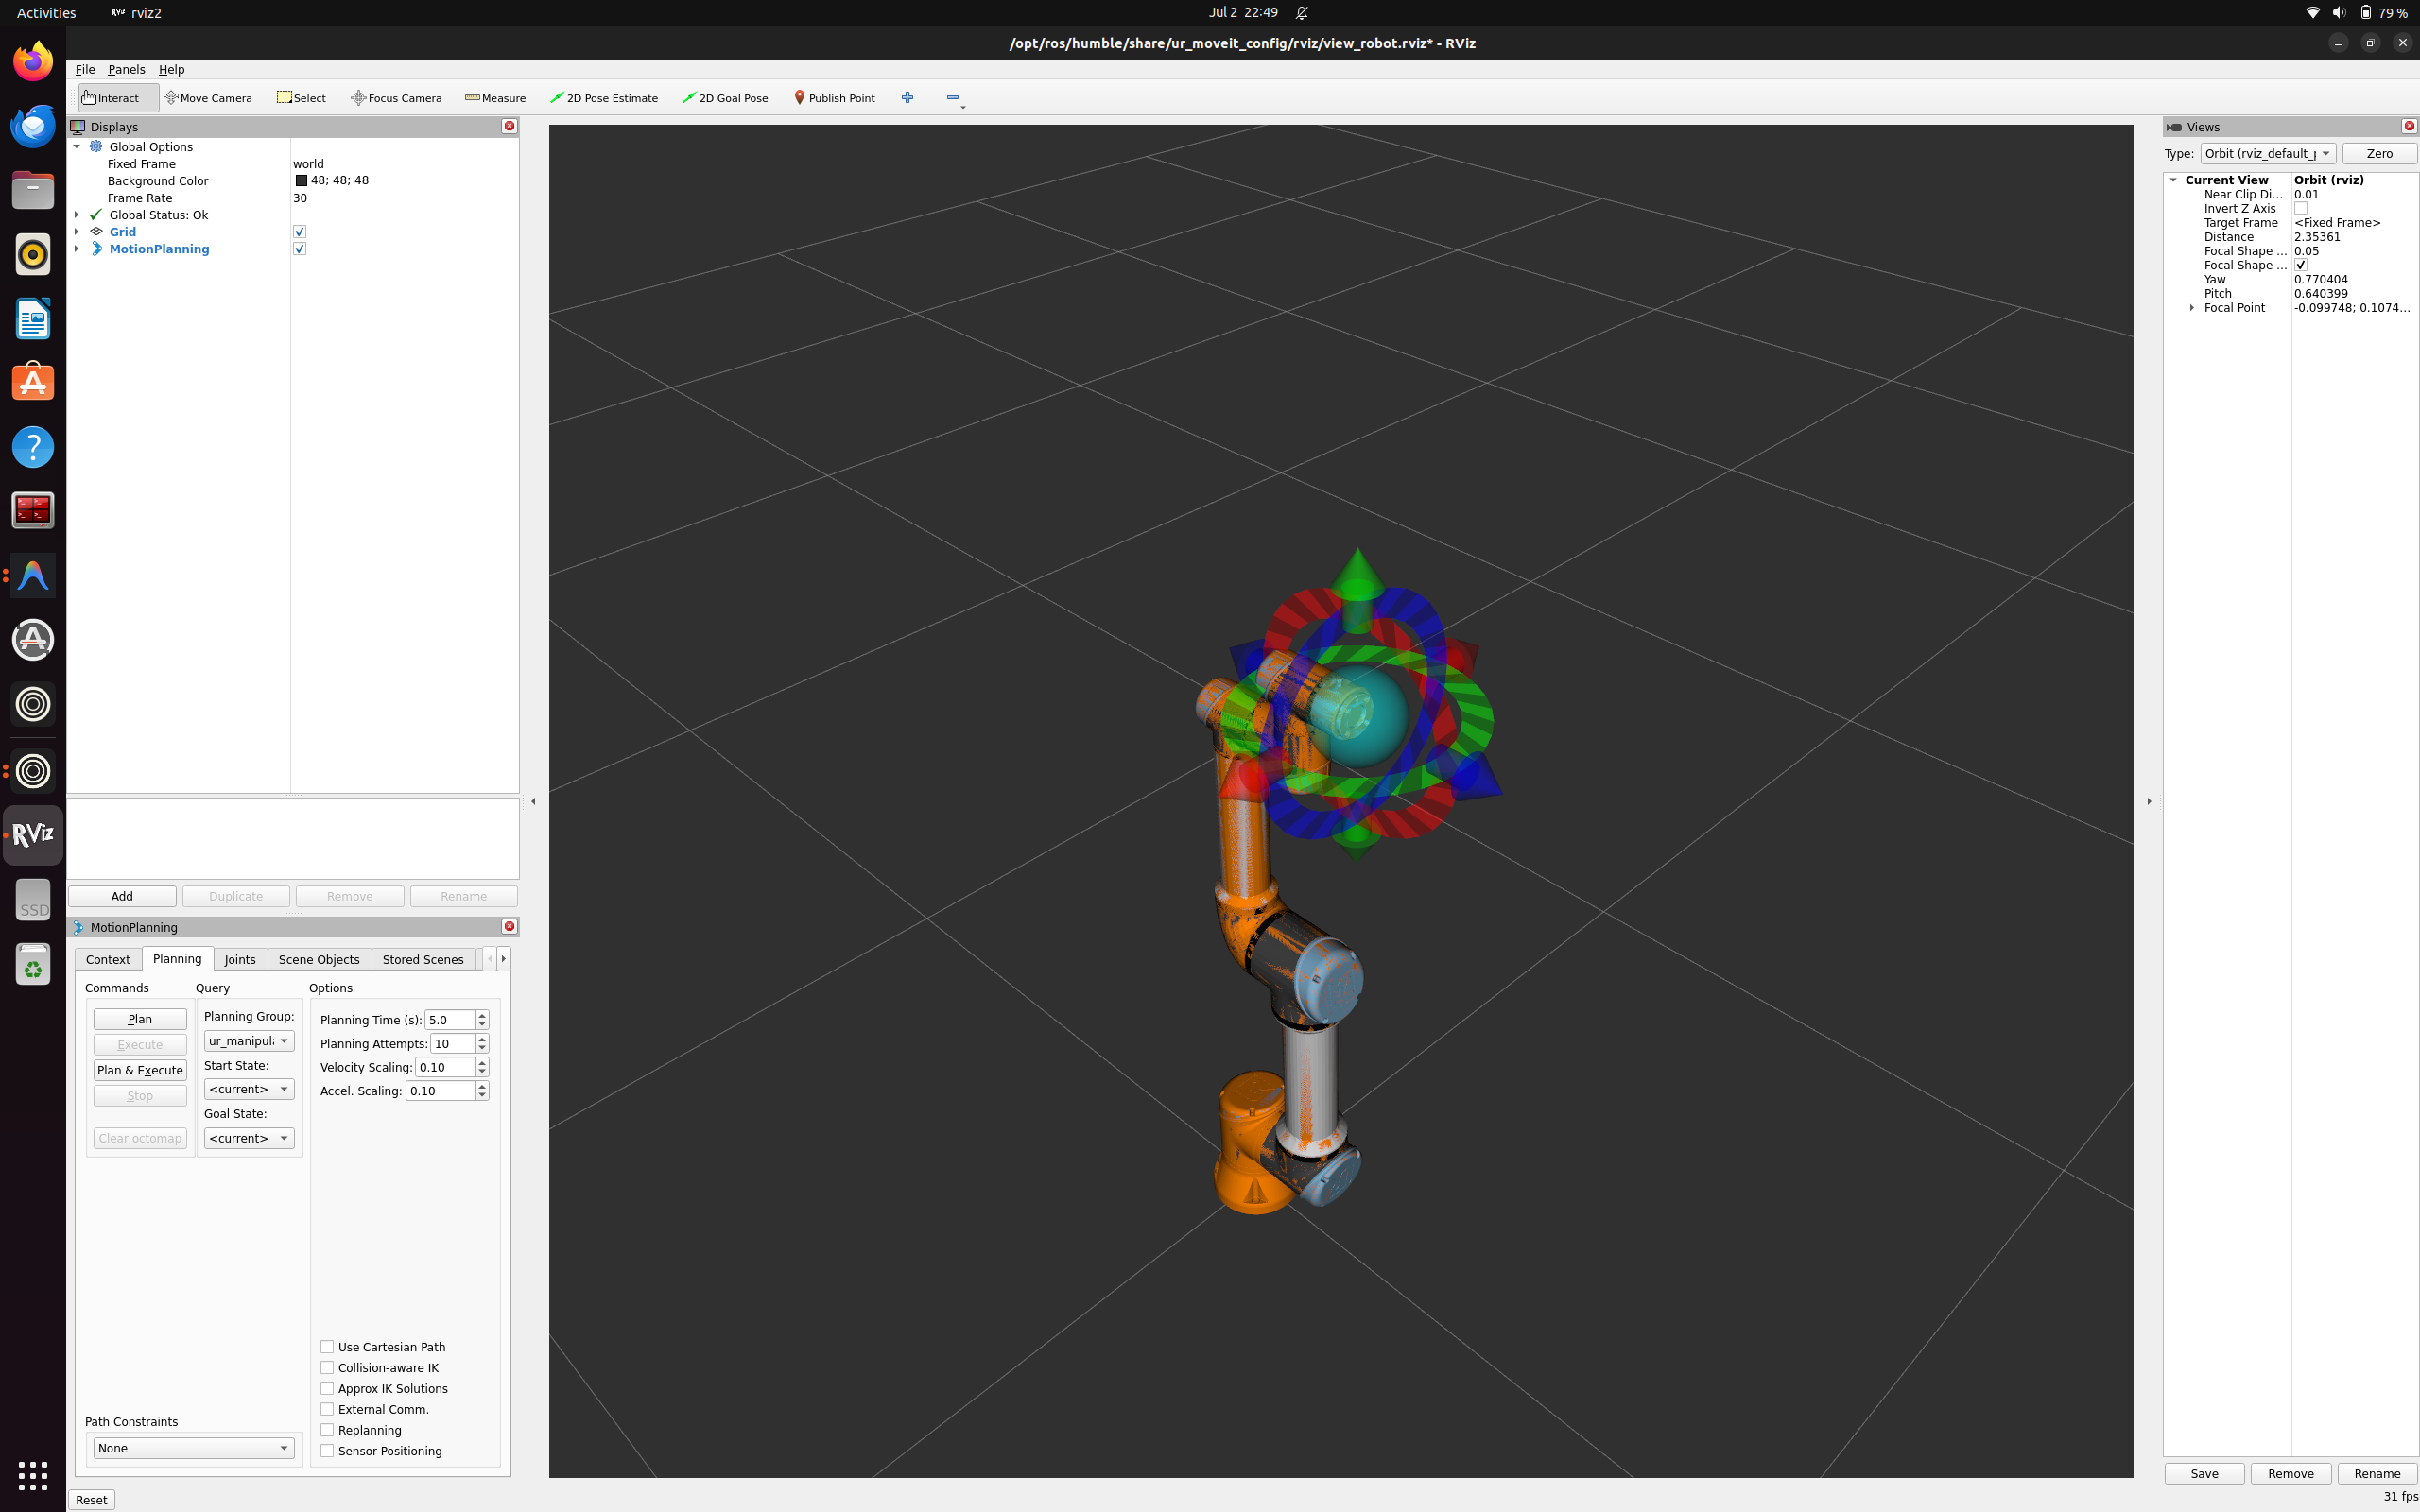
\includegraphics[width=0.9\linewidth]{figures/ch02_first_plan.png}
  \caption{First motion plan, 2 July 2026: UR5e on mock hardware inside the devcontainer.
  MoveIt's MotionPlanning panel with the \texttt{ur\_manipulator} group; the interactive
  marker (rings and sphere) sets the \texttt{tool0} goal pose. Velocity and acceleration
  scaling deliberately at 0.10 --- competition speed comes later, correctness comes first.}
  \label{fig:first-plan}
\end{figure}
